% Made up for the tikra benchmark.
\pgfplotsset{compat=1.18}
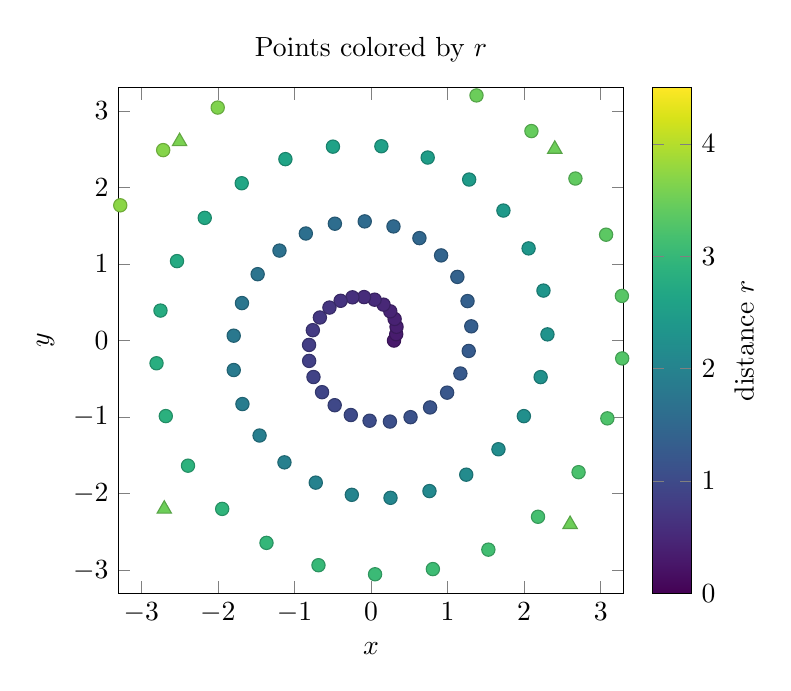
\begin{tikzpicture}
\begin{axis}[width=10.5cm, height=8cm, xmin=-3.3, xmax=3.3, ymin=-3.3, ymax=3.3,
    axis equal image, colorbar, colormap/viridis, point meta min=0, point meta max=4.5,
    colorbar style={ylabel={distance $r$}}, xlabel=$x$, ylabel=$y$, title={Points colored by $r$}]
  \addplot[scatter, only marks, mark=*, mark size=2.4pt, point meta={sqrt(x^2+y^2)},
      samples=90, domain=0:1260, variable=\t]
    ({(0.3+\t/360)*cos(\t)}, {(0.3+\t/360)*sin(\t)});
  \addplot[scatter, only marks, mark=triangle*, mark size=3pt, point meta=explicit]
    coordinates {(-2.5,2.6) [3.6] (2.6,-2.4) [3.5] (2.4,2.5) [3.5] (-2.7,-2.2) [3.5]};
\end{axis}
\end{tikzpicture}
